\section{Post-Training: Expert Model Iteration}

We divide the post-training process into two distinct stages. In stage 1 (\emph{Expert Training}), we construct expert models specializing in three domains: Reasoning, Agent, and General chat. In stage 2 (\emph{Unified Training}), we employ self-distillation techniques to integrate multiple experts, ultimately delivering a comprehensive model capable of generating responses through both deliberative reasoning and direct response modes.

\subsection{Supervised Fine-Tuning}

We perform Supervised Fine-Tuning (SFT) at the beginning of both Stage 1 (\emph{Expert Training}) and Stage 2 (\emph{Unified Training}). In the expert training stage, the primary role of SFT is to provide a cold start, empowering the model with basic chat, reasoning, and tool-use capabilities, which can then be further enhanced in subsequent expert RL training to achieve improved performance. In the unified training stage, the purpose of SFT is to distill the capabilities of different expert models into one hybrid reasoning generalist capable of handling different types of tasks.


\paragraph{Cold Start SFT} During the cold-start phase, we utilize a small set of supervised fine-tuning (SFT) data with extended Chain-of-Thought (CoT) responses. This approach ensures that each expert model possesses adequate foundational ability prior to the reinforcement learning phase.

\paragraph{Overall SFT} In the Overall SFT stage, we collect millions of samples covering reasoning tasks (math, code, science, etc.), general chat (writing, translation, summarization, chit chat, etc.), agentic tasks (basic tool using, coding ability especially for authentic project development, etc.), and long-context understanding tasks from the previously trained expert models, and train the base model with a maximum context length of 128K tokens. By distilling from the output of distinct experts, the model learns to apply the most effective long CoT reasoning for each task to arrive at accurate answers. Especially, recognizing that a prolonged thinking process is unnecessary for certain domains that demand quick responses (such as chit chat), we meticulously balanced training data containing full reasoning with data lacking explicit thought processes. This approach allows the model to operate in both the reflective and immediate response modes, thereby creating a \emph{hybrid reasoning model}. Moreover, we find the following strategy helpful in preparing SFT data to derive optimal performance.

\paragraph{Reducing Character Escaping in Function Call Templates} Although function call parameters are predominantly represented in JSON format in contemporary implementations, a significant challenge emerges when these parameters contain code segments. In such cases, a substantial proportion of characters within the code require escaping, compelling the model to generate extensive escape characters, thereby increasing the learning burden for the model. While this issue poses minimal concern for models primarily designed for general chat, it represents a non-trivial challenge for agentic foundation models where function calling is a core capability.
To mitigate this limitation, we propose a novel function call template that encapsulates function call keys and values within XML-like special token tags. This approach substantially reduces the necessity for character escaping in code segments, as the vast majority of code can be represented in its native form without escaping. Experimental results demonstrate that the proposed function call template does not compromise the performance of function call execution while recucing escaping. The following example (Figure \ref{fig:fc-template}) illustrates the structure of our proposed function call template. Detailed code implementation can be found in our open-source repository.

\begin{tcolorbox}[left=0mm,right=0mm,top=0mm,bottom=0mm,boxsep=1mm,arc=0mm,boxrule=0pt, frame empty, breakable]
\scriptsize
\begin{lstlisting}
<|system|>
# Tools

You may call one or more functions to assist with the user query.

You are provided with function signatures within <tools></tools> XML tags:
<tools>
{"name": "get_weather", "description": "Get the weather of a city for a specific date.", "parameters": {"type": "object", "properties": {"city": {"type": "string", "description": "The city to get weather for, in Chinese."}, "date": {"type": "string", "description": "The date in YYYY-MM-DD format."}}, "required": ["city"]}}
</tools>

For each function call, output the function name and arguments within the following XML format:
<tool_call>{function-name}
<arg_key>{arg-key-1}</arg_key>
<arg_value>{arg-value-1}</arg_value>
<arg_key>{arg-key-2}</arg_key>
<arg_value>{arg-value-2}</arg_value>
...
</tool_call><|system|>
You are a helpful assistant.<|user|>
Today is June 26, 2024. Could you please check the weather in Beijing and Shanghai for tomorrow<|assistant|>
<think>The user wants to check the weather of Beijing and Shanghai tomorrow. I need to call the get_weather function respectively to check Beijing and Shanghai.</think>
I will call the get_weather function to check the weather in Beijing and Shanghai.
<tool_call>get_weather
<arg_key>city</arg_key>
<arg_value>Beijing</arg_value>
<arg_key>date</arg_key>
<arg_value>2024-06-27</arg_value>
</tool_call>
<tool_call>get_weather
<arg_key>city</arg_key>
<arg_value>Shanghai</arg_value>
<arg_key>date</arg_key>
<arg_value>2024-06-27</arg_value>
</tool_call><|observation|>
<tool_response>
{"city": "Beijing", "date": "2024-06-27", "weather": "Sunny", "temperature": "26C"}
</tool_response>
<tool_response>
{"city": "Shanghai", "date": "2024-06-27", "weather": "Overcast", "temperature": "29C"}
</tool_response><|assistant|>
<think>I have obtained the weather query results of get_weather for Beijing and Shanghai respectively and can reply to users directly.</think>
It will be sunny in Beijing tomorrow with a temperature of 26 degrees Celsius. The weather in Shanghai is overcast with a temperature of 29 degrees Celsius.<|user|>
\end{lstlisting}
\end{tcolorbox}
\noindent\begin{minipage}{\textwidth}
\captionof{figure}{One example of function call template.}
\label{fig:fc-template}
\end{minipage}


\paragraph{Rejection Sampling} When sampling from expert models, we employ a comprehensive multistage filtering pipeline that includes: (1) removing repetitive, excessively short, or truncated samples, as well as those that fail to conform to valid reasoning formats; (2) conducting correctness verification for samples with objective answers; (3) utilizing reward models to filter responses to subjective questions; and (4) for tool-calling scenarios, ensuring adherence to proper tool invocation protocols and verification that trajectories reach the expected terminal states.

\paragraph{Prompt Selection and Response-Level Scaling} Filtering challenging prompts and conducting response scaling on them prove to be effective. We experimented with removing the prompts in the bottom 50\% based on response lengths, resulting in a 2\%-4\% improvement in math and science tasks, despite training with only half the data. Notably, we found that applying response scaling to these hard prompts can lead to further gains. Generating four responses for each prompt brought an additional 1\%-2\% improvement.

\paragraph{Automatic Agentic SFT Data Construction} The construction of agentic SFT data involves four steps: 1. \emph{Agentic Framework and Tool Collection}: We gather a set of agentic frameworks and real-world tool APIs and MCP servers, while also leveraging LLMs to automatically construct and simulate a batch of tools. 2. \emph{Task Synthesis}: Based on these frameworks and tools, we automatically synthesize a collection of agentic tasks. On the one hand, for relatively mature frameworks, we leverage LLMs to comprehend their functionalities and automatically generate relevant queries or tasks. On the other hand, for more fragmented or disparate tools, we first select a representative subset and similarly employ LLMs to construct tasks about this subset. These tasks encompass both single-step and multi-step tool calling scenarios. 3. \emph{Trajectory Generation}: For each synthesized task, we utilize existing LLMs to generate tool-call trajectories. Additionally, by employing the LLM as a user simulator, multi-step tool-call tasks are converted into trajectories involving multiple rounds of dialogue. 4. \emph{Quality Filtering}: For each trajectory, multiple judge agents are used to evaluate whether the task is completed. Only successful trajectories are retained.

% \subsection{Reinforcement Learning}

% Our reinforcement learning (RL) algorithm builds upon the GRPO~\cite{shao2024deepseekmath} algorithm without the KL loss term. As outlined in the previous pipeline, we classify RL into three categories: Reasoning RL, Agentic RL, and General RL. The classifications are based on the following criteria: 
% \begin{itemize}
%     \item \textbf{Reasoning RL} is characterized by its reasoning-intensive nature and ease of verification. For example, tasks such as solving mathematical problems (excluding proof-based problems, which will apparently become one of our future directions), or executing code to test its functionality fall under this category. The rewards in these tasks are highly precise, as correctness can be determined with clarity and accuracy. 
%     \item \textbf{Agentic RL}...
%     \item \textbf{General RL} covers a wide range of domains, such as writing, instruction following, function calling, and long-context comprehension. In these tasks, answers are harder to validate, and the definition of rewards tends to be more ambiguous.
% \end{itemize}

% Recognizing the fundamental differences among these RL types, we have developed task-specific training approaches tailored to each category, discussed in the following subsections.

\subsection{Reasoning RL}

Reasoning RL focuses on enhancing a model's capabilities in domains that demand logical deduction, structured problem-solving, and verifiable accuracy. This includes critical areas such as mathematics, code generation, and scientific reasoning. A defining characteristic of these tasks is the high precision of their reward signals, as correctness can often be determined programmatically or with objective clarity. Mastery in these areas is not only crucial for advancing the raw intelligence of models but also serves as a fundamental building block for more complex, multi-step agentic behaviors. Recognizing the unique challenges and opportunities within reasoning RL, we have developed a suite of specialized techniques to effectively train our models. These methods, detailed below, are designed to address issues such as training efficiency, sample diversity, and data quality. Our overall RL algorithm builds upon the GRPO~\cite{shao2024deepseekmath} framework, excluding the KL loss term. The comparison curves shown in this section are based on our smaller experimental model, not on GLM-4.5.


\begin{figure}[t]
    \centering
    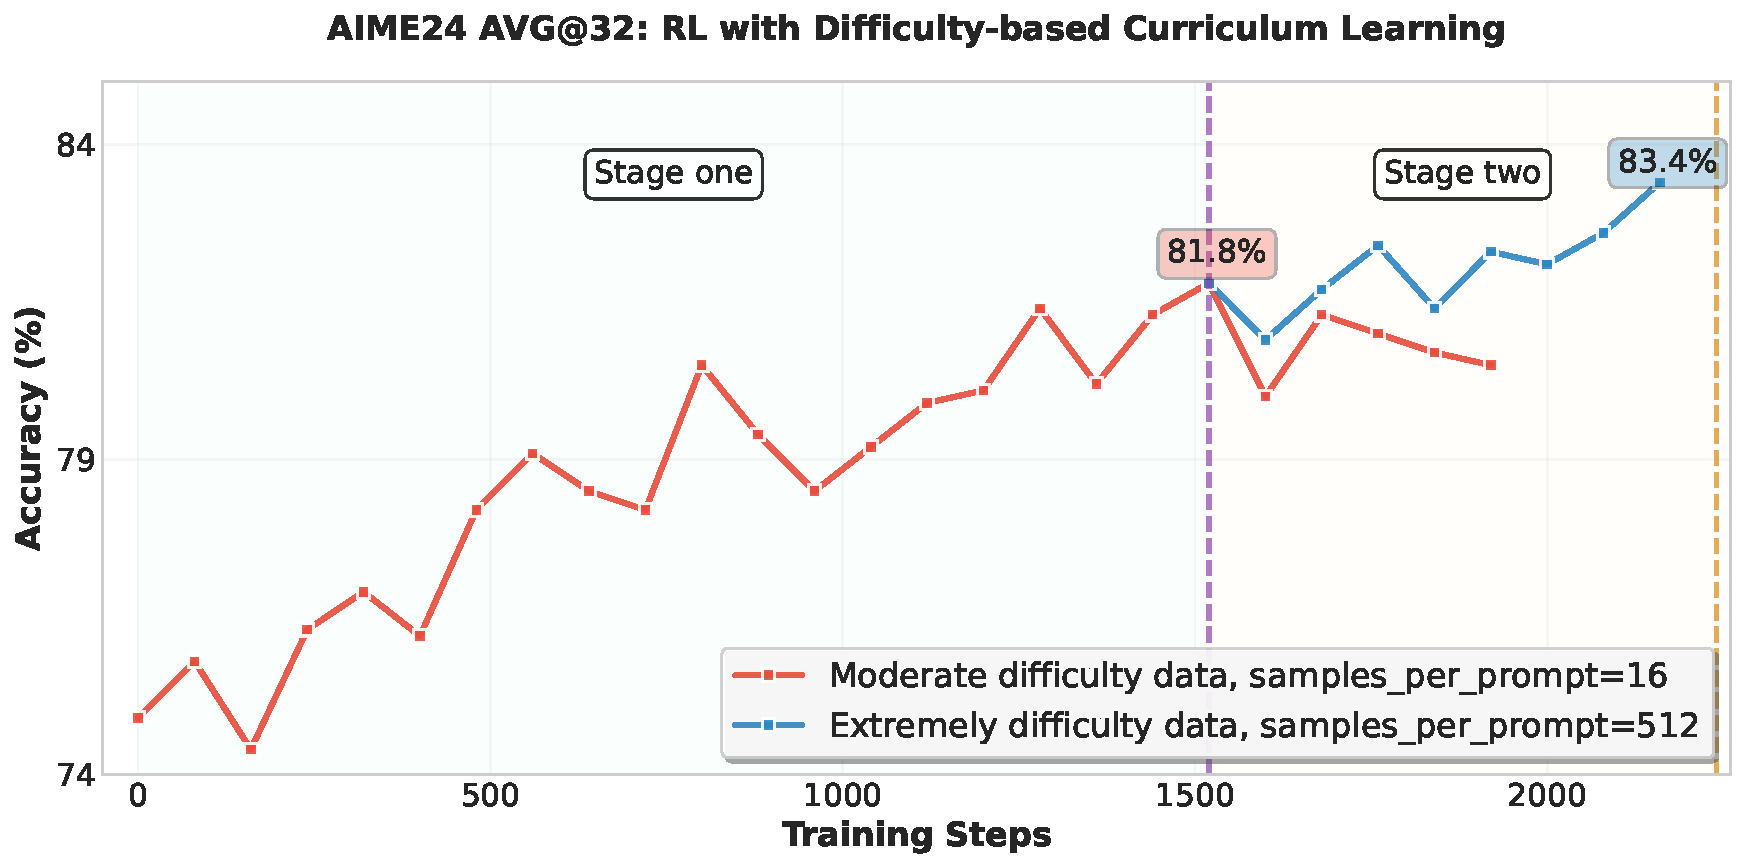
\includegraphics[width=0.85\textwidth]{figures/curriculum_rl.pdf}
    \caption{\textbf{Effectiveness of the two-stage difficulty-based curriculum on AIME'24.} The \textcolor{blue}{blue line} (our method) switches to extremely difficult problems (pass@8$=$0, pass@512$>$0) in the second stage, showing continued improvement. The \textcolor{red}{red line} (baseline) continues with moderate-difficulty problems and plateaus.}
    \label{fig:curriculum_rl}
\end{figure}

\paragraph{Difficulty-based Curriculum Learning}
During reinforcement learning, the model's proficiency evolves, creating a mismatch with static training data. In the later stages, as the model becomes more capable, overly simple data can lead to rollouts where all rewards are 1s. Conversely, in the early stages, excessively difficult data often results in batches where all rewards are 0s. In both scenarios, the lack of reward variance provides no useful gradient signal, severely hindering training efficiency. To address this challenge, we employ a two-stage difficulty-based curriculum for RL. The effectiveness of this and other strategies discussed below is validated through controlled experiments on a smaller model, which allows for rapid iteration and precise ablation studies. As shown in Figure~\ref{fig:curriculum_rl}, this two-stage approach enables the model to consistently surpass its performance ceiling. Crucially, to maintain high signal quality and reduce noise, all problems used in the second stage are strictly sourced from a pool with verified correct answers.




\begin{figure}[t]
    \centering
    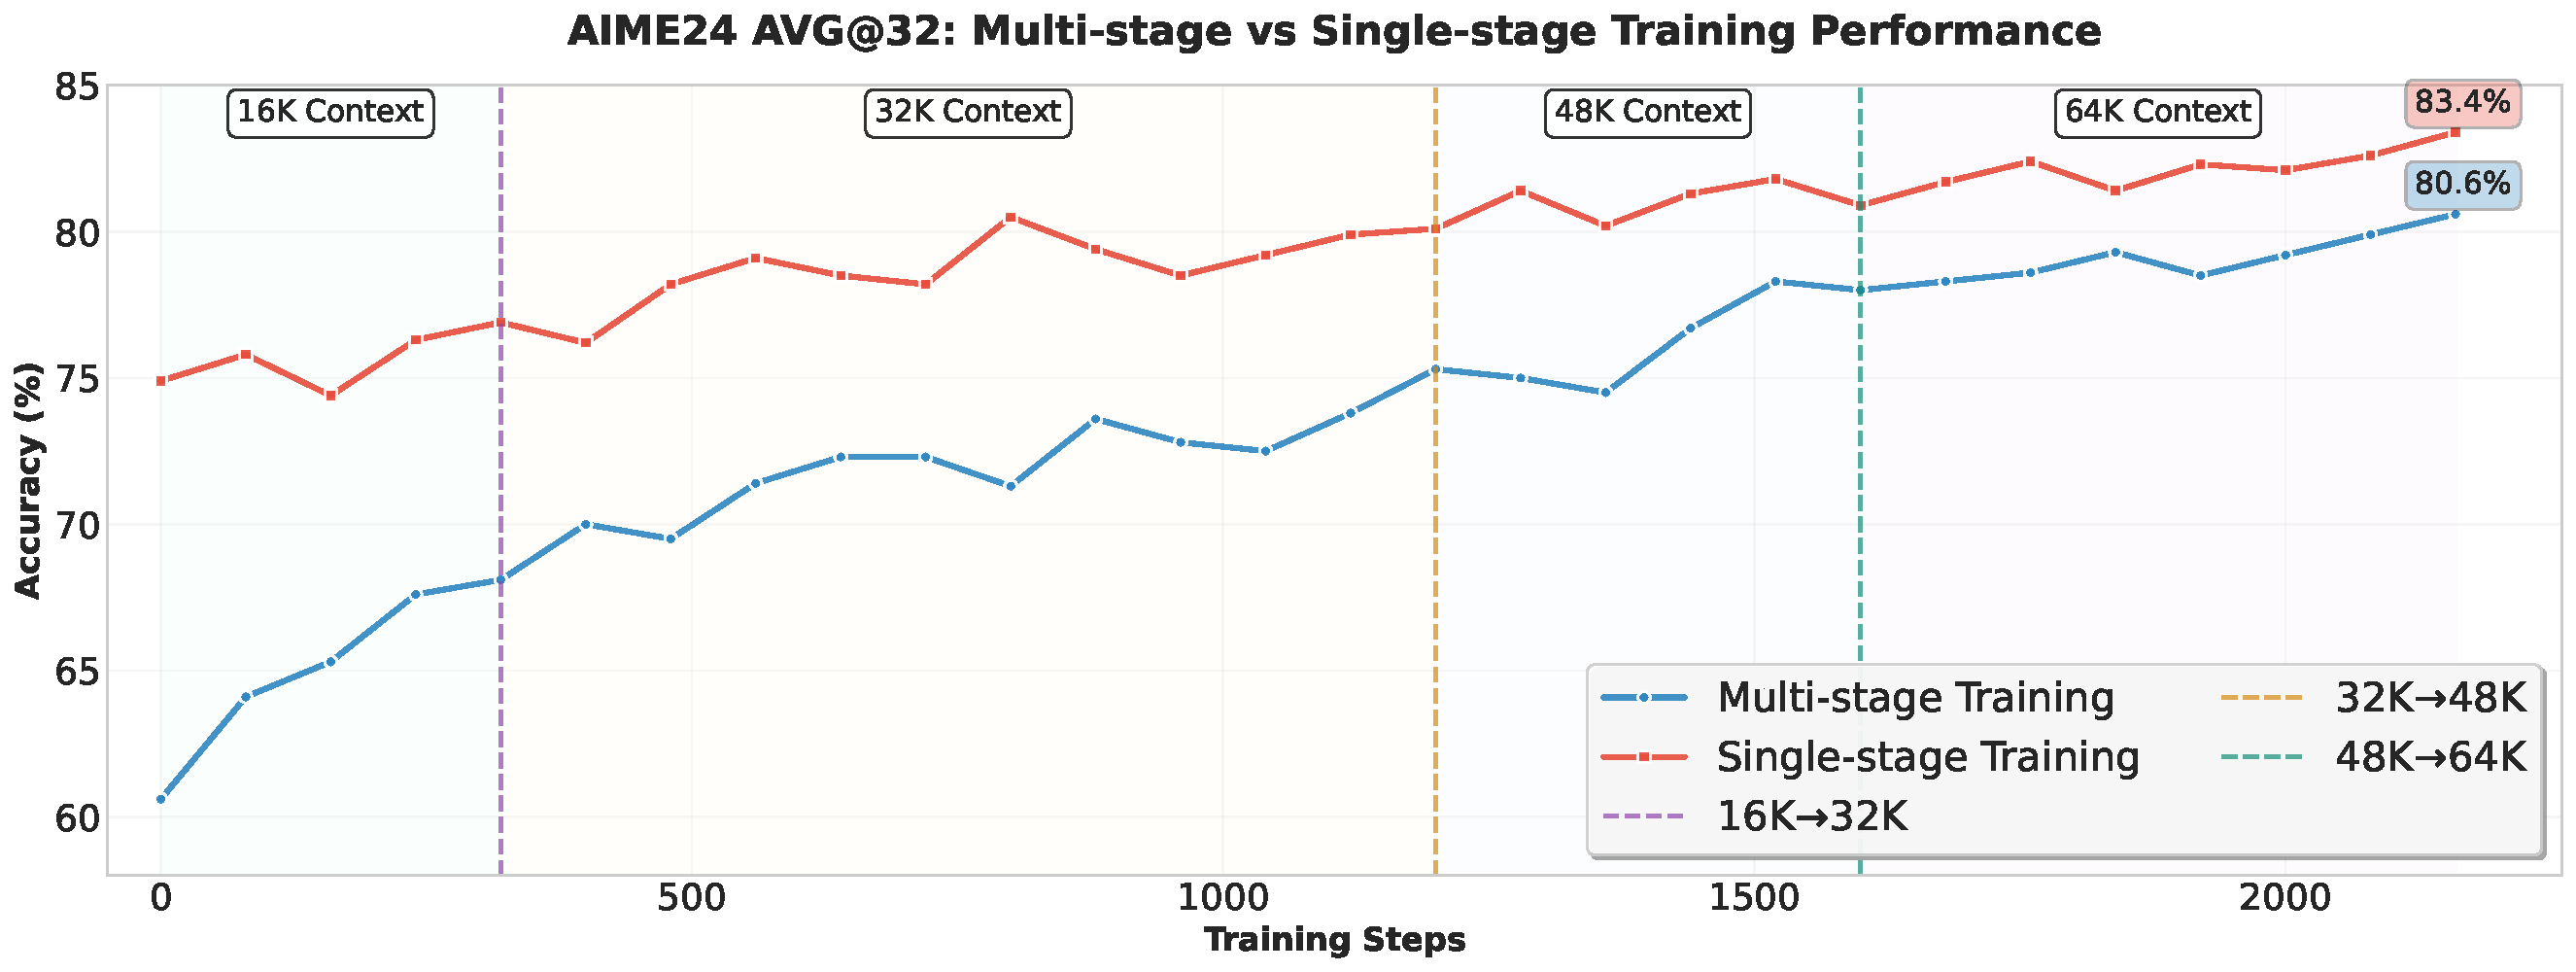
\includegraphics[width=1.0\textwidth]{figures/multi_stage_rl.pdf}
    \caption{\textbf{Single-stage vs. multi-stage RL at 64K context length.} The \textcolor{red}{red line} (single-stage at 64K) achieves superior performance. The \textcolor{blue}{blue line} (multi-stage with progressively increasing length) suffers from an irreversible performance drop in early stages, limiting its final performance.}
    \label{fig:single_stage_rl}
\end{figure}

\paragraph{Single-Stage RL at 64K Output Length}
Previous research~\cite{deepscaler2025} has suggested conducting RL in multiple stages with progressively increasing maximum output lengths. However, our experiments reveal that this multi-stage approach is less effective than a single-stage RL process conducted directly at the maximum target length of 64K. Since the initial Supervised Fine-Tuning (SFT) has already conditioned the model on generating 64K-length responses, introducing RL stages with shorter maximum lengths can cause the model to ``unlearn'' its long-context capabilities. This often leads to a significant and irreversible drop in performance, as the model's average output length decreases. This degradation is difficult to recover from in the final 64K-length RL stage, thus limiting further improvement. Our experiments confirm this observation: as demonstrated in Figure~\ref{fig:single_stage_rl}, applying RL directly at the full 64K-length continually pushes the model's limits and yields better performance.

\paragraph{Dynamic Sampling Temperature}
During RL, the sampling temperature is a key parameter for controlling trajectory diversity. A temperature that is too low leads to convergent, less exploratory outputs, while one that is too high introduces low-quality, noisy samples, undermining both model accuracy and training efficiency. Using a fixed sampling temperature is suboptimal because it fails to adapt as the policy distribution becomes more concentrated (i.e., has lower entropy), often resulting in insufficient exploration at later stages. Therefore, we propose dynamically adjusting the sampling temperature to maintain a healthy balance between accuracy and exploration. Specifically, when the average reward of rollouts stabilizes, we identify this as a convergence phase and increase the sampling temperature to encourage greater diversity. To mitigate the risk of introducing excessive noise, we implement a quality-control mechanism: we periodically evaluate model performance on a held-out validation set across a range of temperatures. The temperature for the next training phase is then set to the maximum value that does not cause a performance drop of more than 1\% from the current optimum~\cite{Polaris2025}.


\begin{figure}[t]
    \centering
    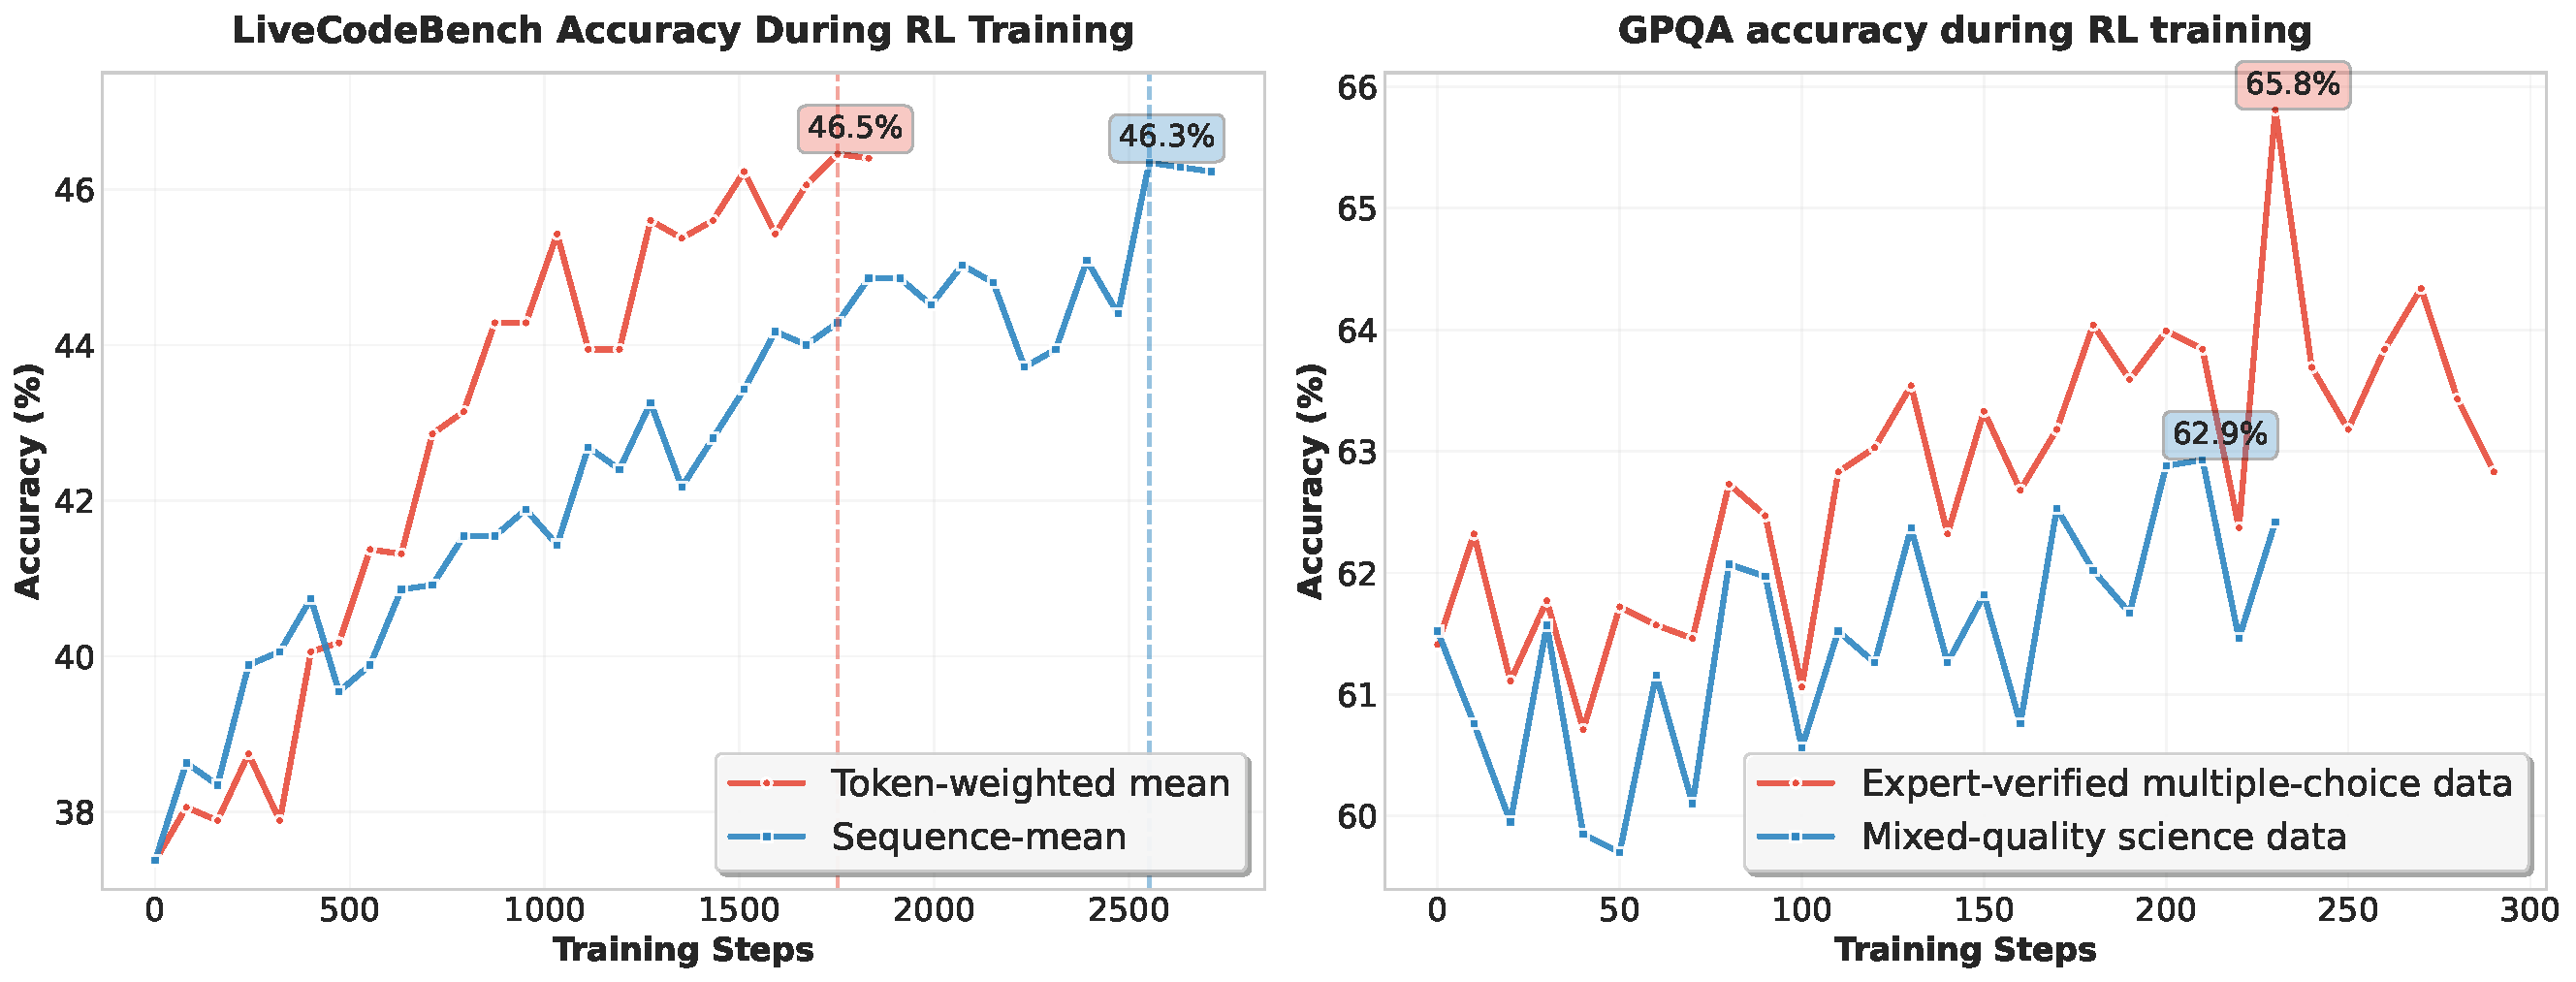
\includegraphics[width=1.0\textwidth]{figures/code_science.pdf}
    \caption{\textbf{Ablation Studies for Code and Science RL.} 
    \textbf{(Left)} Comparison of loss calculation methods for code RL. The \textcolor{red}{token-weighted mean loss} approach achieves faster convergence compared to the \textcolor{blue}{sequence-mean loss} baseline, accelerating the training process. 
    \textbf{(Right)} Ablation on data sources for science RL on the GPQA-Diamond benchmark. Training exclusively on a small set of high-quality, expert-verified multiple-choice questions yields the best performance, significantly outperforming training on mixed-quality data.}
    \label{fig:code_science_rl}
\end{figure}


\paragraph{Code and Science RL}
Compared to mathematics, RL for coding and scientific domains has received less attention in the literature. We conducted extensive controlled RL experiments in these areas and arrived at the following empirical conclusions. For \textbf{code RL}, we find that the choice of loss calculation is critical for training efficiency. As illustrated in Figure~\ref{fig:code_science_rl} (left), adopting a token-weighted mean loss is highly beneficial compared to a conventional sequence-mean loss. The token-weighted approach provides a finer-grained and more stable gradient signal, which leads to significantly faster convergence. This method also helps to alleviate the length bias inherent in sequence-level rewards and effectively suppresses the generation of overly simplistic or repetitive ``base case'' samples during training. For \textbf{science RL}, our findings on the GPQA-Diamond benchmark highlight that data quality and type are paramount factors. As shown in Figure~\ref{fig:code_science_rl} (right), using exclusively expert-verified multiple-choice questions for RL leads to significantly better performance compared to training with mixed-quality or unverified data. This result underscores that even for tasks with simple formats like multiple-choice, rigorously filtering the RL data pool to include only high-quality, challenging instances is crucial for effective model improvement.






\subsection{Agentic RL}

Reinforcement Learning from Human Feedback (RLHF) helps language models follow human instructions more faithfully. Applying RL to math and programming contests has further uncovered strong reasoning abilities and favorable scaling behavior on tasks whose outcomes can be objectively verified. Building on these insights, we focus on agentic settings—specifically web-search and code-generation agents—where every action or answer can be automatically checked. This built-in verifiability supplies dense, reliable rewards, enabling us to scale RL training more effectively.


\subsubsection{Data Collection and Synthesis for Agents}


For web‑search tasks and open‑domain information seeking, we develop a data‑synthesis pipeline that yields demanding question–answer pairs requiring multi‑step reasoning across multiple web sources. This corpus is designed to sharpen GLM’s ability to uncover elusive, interwoven facts on the internet. Dataset construction blends two approaches: (1) an automated pipeline powered by multi‑hop reasoning over knowledge graphs, and (2) human‑in‑the‑loop extraction and selective obfuscation of content from several web pages to prepare reinforcement‑learning training signals.


For software‑engineering tasks, we curate an extensive collection of GitHub pull requests and issues to create a realistic software‑development benchmark comprising user prompts and executable unit tests. All evaluations run inside a hardened sandbox with a distributed system, which provides both horizontal scalability and strong isolation guarantees.

\subsubsection{Pushing the Limits with Reinforcement Learning and Iterative Self-distillation}

We adopt the group-wise policy optimization algorithm for RL training.
For each problem \(x\), we sample \(K\) agent traces \(\{y_1,\dots,y_k\}\) from the previous policy
\(\pi_{\text{old}}\), and optimize the model \(\pi_\theta\) with respect to the following objective:
\[
L_{\text{RL}}(\theta)
   = \mathbb{E}_{x\sim\mathcal{D}}\!\left[
        \frac{1}{K}\sum_{i=1}^{K}
        \left(
            r(x,y_i) - \bar{r}(x)
        \right)
     \right],
\]
where $\bar{r}(x) \;=\; \frac{1}{k}\sum_{i=1}^{k} r\bigl(x,y_i\bigr)$
is the mean reward of the sampled responses. It is noted that only model-generated tokens are used for optimization, and the environment feedback is ignored in loss computation. 

\paragraph{Outcome Supervision with Process Action Format Penalty} For web search tasks, we use the accuracy of the final answer as a reward for the entire agent trace. For coding agents, we primarily utilize SWE data with verifiable test cases for RL training. Our experiments have shown that RL training on web search and SWE tasks leads to generalized performance improvements across other tasks and benchmarks, such as general tool usage and coding tasks like Terminal-Bench. Additionally, we apply a process format penalty to ensure the model generates correct tool call formats. If the model fails to produce the correct tool format during agent trace generation, the process will be halted, and the trace will receive a zero reward.

\paragraph{Iterative Distillation} Since RL training on agent tasks is time-consuming, we adopt a self-distillation approach to iteratively enhance the performance of the SFT cold-start model before resuming RL training on this improved model. Specifically, we first perform RL training on the initial cold-start model to boost agent performance. Once training has reached a certain step count or plateaued, we apply self-distillation by substituting the original cold-start data with responses generated by the RL-trained model, thus creating a superior SFT model. We then conduct further RL training on this enhanced model, progressively increasing training difficulty. This iterative strategy allows us to push the performance limits of RL-trained models efficiently.

\paragraph{Scaling Test-time Compute via Interaction Turns} For agent tasks, we observe significant performance gains given increasing interaction turns with the environment. Compared to test-time scaling in reasoning models, which scales output tokens, agent tasks make use of test-time compute by continuously interacting with the environment, e.g., searching high and low for hard-to-find web information or writing test cases for self-verification and self-correction for coding tasks. 
Figure~\ref{fig:turn_scaling} shows that with varying browsing effort,  accuracy scales smoothly with test-time compute.

\begin{figure}[t]
    \centering
    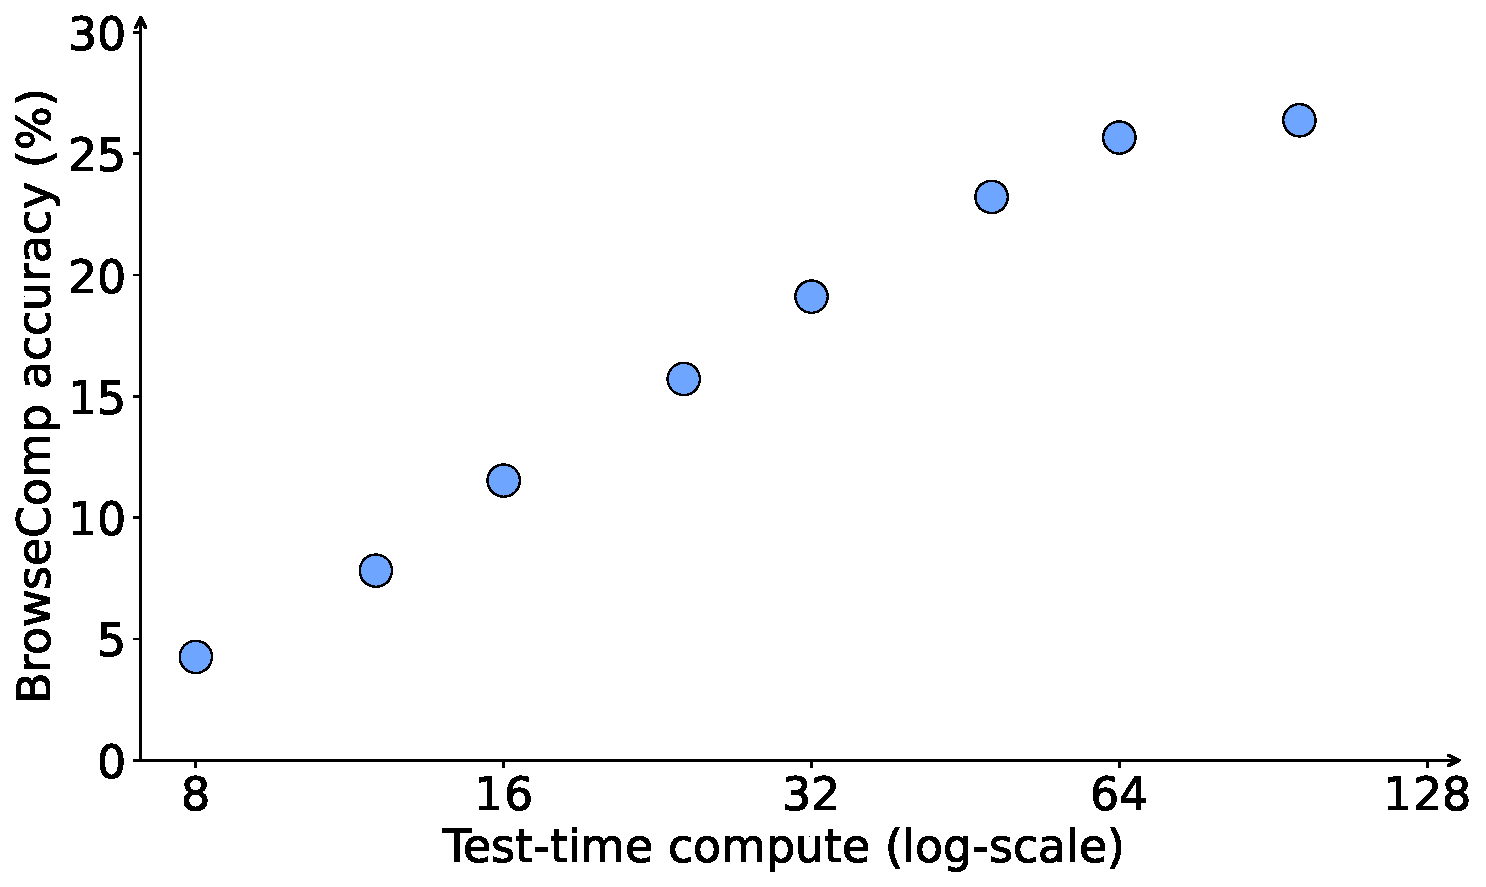
\includegraphics[width=0.6\linewidth]{figures/browsecomp-360b-sft-scaling-log.pdf}
    \caption{Interaction Turns Scaling for BrowseComp. }
    \label{fig:turn_scaling}
\end{figure}







\subsection{General RL}

General RL aims to holistically improve the model's overall performance, remediate potential issues, and strengthen key capabilities. Central to our methodology is a multi-source feedback system that synergizes rule-based feedback, human feedback (RLHF), and model-based feedback (RLAIF). This hybrid framework provides more robust training signals and allows us to leverage the unique advantages of each source: the precision of automated rules, the nuanced judgment of human annotators, and the scalability of AI-driven evaluation.

\paragraph{Holistic RL}

Holistic RL targets broad performance gains across diverse domains. To this end, we first construct a balanced dataset of roughly 5,000 prompts spanning 7 primary, 33 secondary, and 139 tertiary categories.
Reward signals for Holistic RL are derived from both human and AI feedback. For human feedback, we train a reward model on preference annotations. 
% This was achieved by presenting human annotators with model-generated responses and asking them to provide preference labels based on a comprehensive evaluation of multiple dimensions, such as instruction following, safety, and factual correctness. 
Annotators compare model responses and assign preference labels based on a comprehensive evaluation of multiple dimensions, such as instruction following, safety, and factual correctness.
For model feedback, we design separate scoring rubrics that depend on whether the prompt has an objective ground-truth answer.
Merging the two feedback sources yields more reliable and expressive reward signals, mitigating the inherent limitations of each individual method.

\paragraph{Instruction Following RL}

Instruction Following RL improves the model’s ability to understand and satisfy complex instructions. To achieve this, we create a fine-grained taxonomy with 7 major and 151 minor constraint types, covering content requirements, formatting rules, and more. Based on this taxonomy, a dedicated training set of challenging instructions is assembled to cover every constraint type.
The feedback system consists of deterministic verification rules, a trained reward model, and a critique model. The robustness of this hybrid feedback system proves crucial during GRPO training. We observe mitigated reward hacking, enabling the policy model to achieve continuous and steady improvements in instruction following as shown in Figure~\ref{fig:instruction-following-RL}.

\begin{figure}[t]
    \centering
    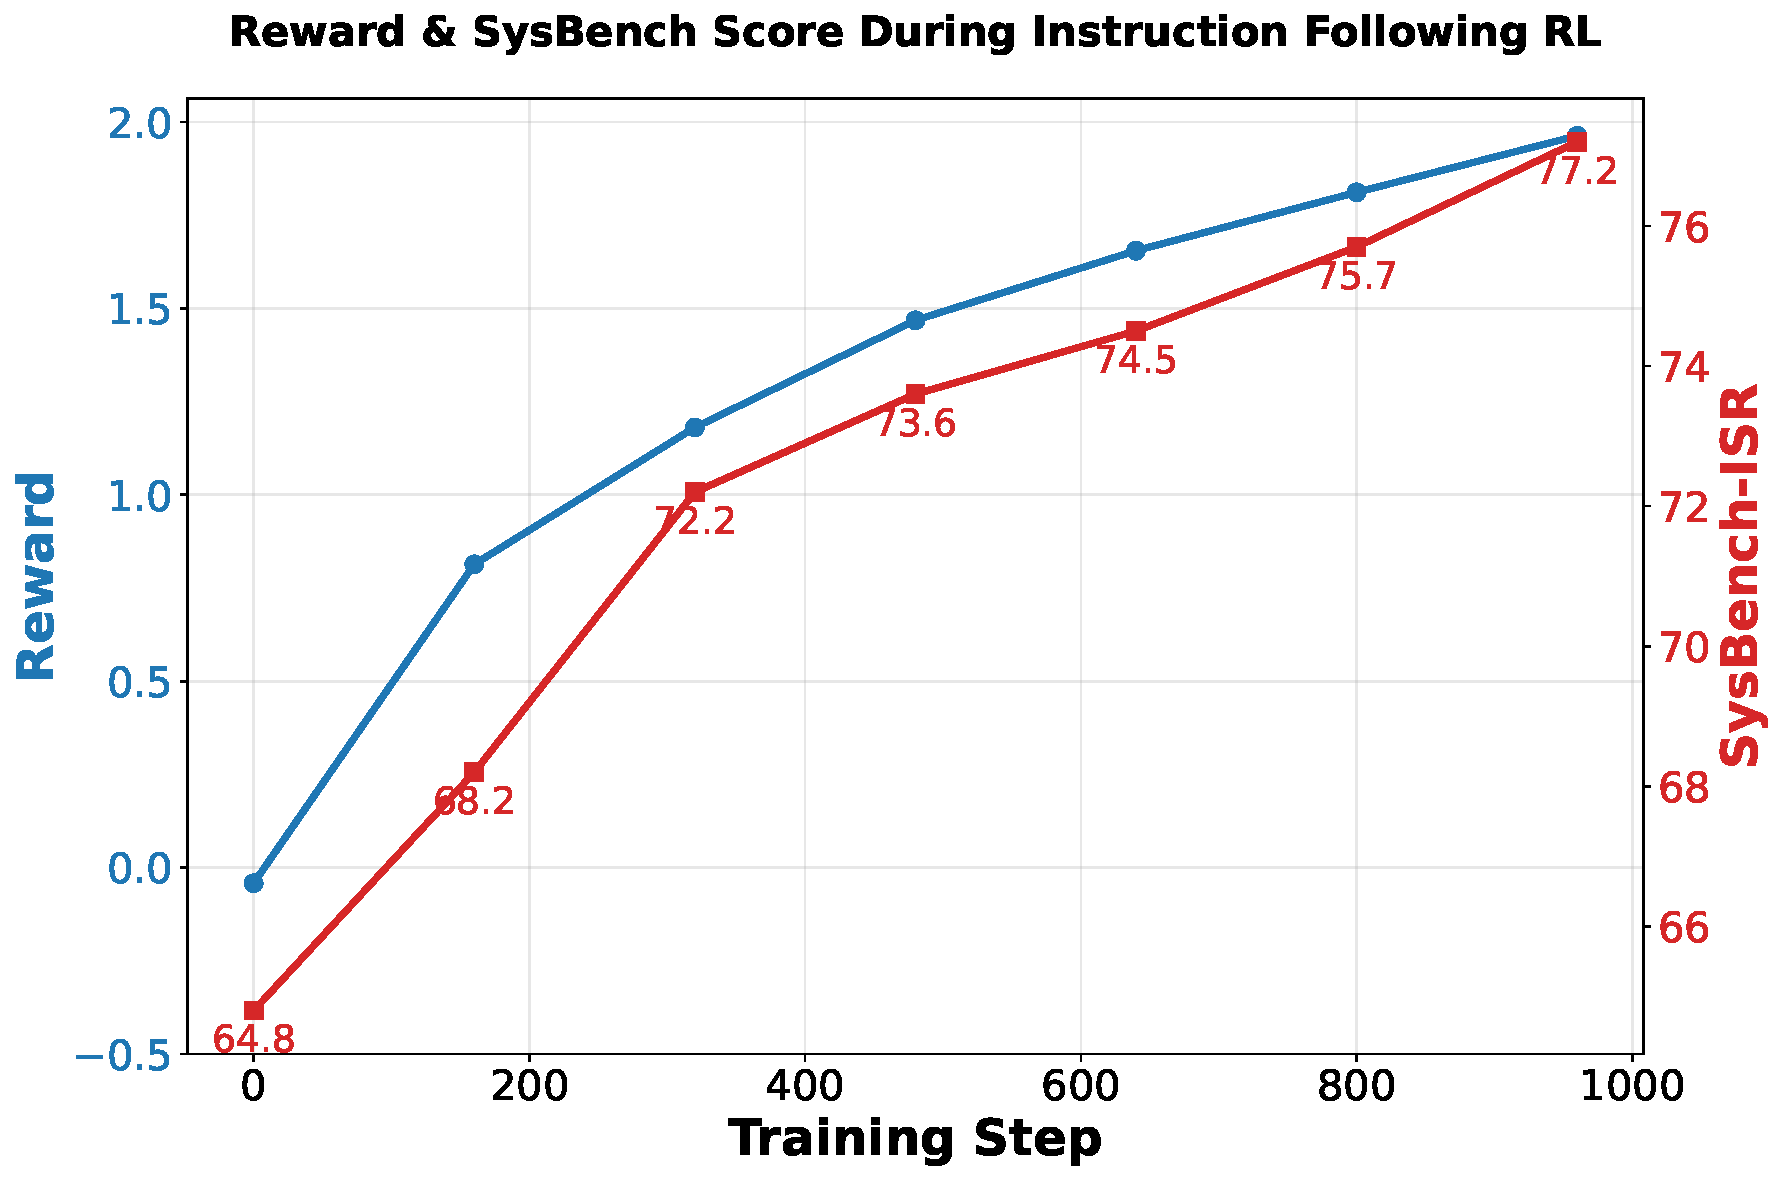
\includegraphics[width=0.65\linewidth]{figures/reward_sysbench_isr_curve.pdf}
    \caption{\textbf{Training curve of Instruction Following RL without other General RL tasks.} During GRPO training, the instruction following performance (\textcolor{red}{SysBench-ISR}) improves in step with the increasing \textcolor{blue}{reward}. Up to roughly 1,000 training steps, we have not observed clear evidence of reward hacking.}
    \label{fig:instruction-following-RL}
\end{figure}


\paragraph{Function Calling RL}
Function Calling RL is divided into step-wise rule-based RL and end-to-end multi-turn RL. We incorporate step-wise rule-based RL directly into our general RL framework due to their similar output lengths and convergence speeds. For end-to-end multi-turn RL, we first train specialized expert models and then distill these experts into the main model.

\begin{itemize}[leftmargin=*,itemsep=0pt,topsep=0pt]
    \item \textbf{Step-wise Rule-based RL}: For tasks with clear tool invocation procedures, we annotate the ground truth function call for each step/turn in the training data. Given the task and the function calls from previous steps/turns, the model is trained to generate the next assistant response, which can be a function call or a response to the user. Using rule-based rewards, we guide the model to make correct function calls over consecutive rounds.
    Accordingly, we design the following strict reward function:
    $$\text{Reward} =
    \begin{cases}
    1, & \text{if } \texttt{FormatCorrect}(a_t)\ \text{and}\ \texttt{Match}(a_t, a_t^*) \\
    0, & \text{otherwise}
    \end{cases}$$
    Here, $a_t$ denotes the t-th function call generated by the model, and $a_t^*$ is the corresponding ground truth function call. A reward of 1 is only given if $a_t$ is in the correct format and matches the ground truth exactly (including the name, parameters, and every field). Otherwise, the reward is 0.
    Such a strict reward rule not only guides the model to generate correct function calls but also strongly enforces output formatting, improving the model’s usability and robustness in real-world interactions.
    \item \textbf{End-to-end Multi-turn RL}: Step-wise rule-based RL decomposes tasks into static, predetermined decision flows. In this process, the model lacks dynamic interactions with the environment and cannot autonomously explore, plan, or handle complex situations, thereby making its real-world problem-solving ability limited. To address these issues, we introduce end-to-end multi-turn function calling RL, where the model first generates the complete trajectory and is then rewarded based on task completion. In this way, the model can optimize its action policy through continuous trial and error with tool feedback, significantly enhancing its ability in autonomous planning and decision-making.
    Specifically, end-to-end multi-turn function calling RL considers two types of complex tasks: 1. single-turn multi-step tasks: The model needs to make multi-step function calls and interact with the environment to complete such tasks. We use complex tasks automatically synthesized based on MCP servers, as well as some open-source agentic datasets with runnable environments, such as Agentgym~\cite{xi2024agentgym}. 2. multi-turn multi-step tasks: Besides interacting with the tool execution environment, the model also needs to interact with an LLM-simulated user agent to obtain complete task information and accomplish the overall task.
    The reward for end-to-end multi-turn function calling RL is computed as:
    $$\text{Reward} =
    \begin{cases}
    1, & \text{if } \texttt{FormatCorrect}(a_1, \dots, a_T)\ \text{and}\ \texttt{TaskCompleted}(I, o_0,a_1, o_1, \dots, a_T,o_T) \\
    0, & \text{otherwise}
    \end{cases}$$
    Here, $I$ refers to the original complex task, $a_t$ is the t-th function call, and $o_t$ is the tool feedback or user information. $\texttt{TaskCompleted}(I, o_0,a_1, o_1, \dots, a_T,o_T)$ indicates whether the task is completed, which is determined by the environment according to predefined rules or by an LLM Judge Agent.
\end{itemize}

\paragraph{Pathology RL}

As the final stage of post-training, general RL needs to rectify potential issues, such as language mixing, excessive repetition, and formatting mistakes. Although penalizing such behaviors in the above-mentioned general RL tasks is effective, the low incidence rate of these pathologies (often less than 1\% of outputs) makes this a sample-inefficient optimization strategy. Therefore, we curate a targeted dataset for pathology RL by identifying prompts that are highly likely to trigger these pathological behaviors.
Training on this dataset lets us impose efficient penalties, further lowering the residual error rates for these problematic behaviors.

\subsection{RL Infrastructure}

\begin{figure}[t]
    \centering
    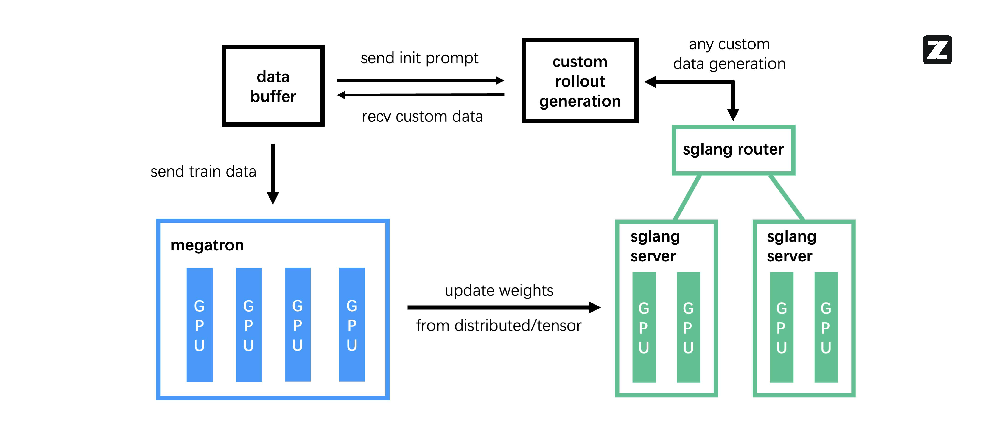
\includegraphics[width=0.9\linewidth, trim=0 10 0 10, clip]{figures/slime}
    \caption{Overview of the Slime RL infrastructure. The system consists of three core modules: \textbf{Training (Megatron)} – handles the main training process, reads data from the Data Buffer, and synchronizes parameters with the rollout module after training; \textbf{Rollout (SGLang + Router)} – generates new data, including rewards and verifier outputs, and writes it to the Data Buffer; \textbf{Data Buffer} – serves as a bridge module that manages prompt initialization, custom data, and rollout generation strategies.}
    \label{fig:slime}
\end{figure}

Our RL infrastructure is built upon Slime\footnote{\url{https://github.com/THUDM/slime}}, an open-source framework we developed. The framework is engineered with several key optimizations to enhance flexibility, efficiency, and extensibility.

\paragraph{Flexible Hybrid Training and Data Generation Architecture} A core feature of our infrastructure is its support for highly flexible training paradigms and data generation strategies within a single, unified system. This design allows us to cater to the distinct requirements of various RL tasks by supporting both a colocated, synchronous mode and a disaggregated, asynchronous mode. This flexibility in data generation is crucial for extending our RL capabilities to new domains and more complex agentic environments.
We observed that different RL tasks benefit from different scheduling approaches. For general-purpose RL tasks or those aimed at enhancing model reasoning capabilities (e.g., in mathematics and code generation), a synchronous, colocated architecture is more effective. In this setup, the training and inference engines reside on the same worker. This, combined with dynamic sampling, significantly reduces GPU idle time and maximizes resource utilization.
Conversely, for agentic tasks, such as those in Software Engineering (SWE), the data generation process is often protracted and involves complex system interactions. To ensure that the agent environments can operate continuously and maximize data throughput, we adopt a disaggregated, asynchronous model. The rollout component of the RL framework is exposed directly to the agent environment, while the GPUs for training and inference are scheduled independently. This decoupling enables the agent environments to constantly generate new data without being stalled by the training cycle.
By leveraging the resource scheduling and asynchronous capabilities of the Ray framework, we can flexibly place the inference and training engines on the same GPU or on different ones. This dual support for synchronous and asynchronous training allows diverse RL tasks to share a common set of underlying optimizations for both training and inference.

\paragraph{Accelerated Rollout with Mixed-Precision Inference} Rollout efficiency is a persistent bottleneck in RL training. To address this, our infrastructure supports BF16 for training while leveraging FP8 for inference to accelerate the data generation phase.
During each policy update iteration, we perform online, block-wise FP8 quantization on the model parameters before they are dispatched for rollout. This dynamic quantization enables highly efficient FP8 inference, significantly improving the overall throughput of the data collection process.


\paragraph{Agent-oriented RL Infra Design}

To conduct RL for agent tasks, we design a fully asynchronous and decoupled RL infrastructure that efficiently handles long-horizon agent rollouts and supports flexible multi-task RL training across diverse agent frameworks.

Agentic rollouts often require prolonged interactions with complex environments, which can significantly slow down the overall RL training process. To overcome this, we first design a high-concurrency Docker-based runtime that provisions isolated environments for each task, drastically reducing rollout overhead. In addition, we implement a fully asynchronous RL training loop. Because agent tasks can vary in type and trajectory length, synchronous RL training often leads to severe GPU underutilization as workers wait for the slowest rollouts to complete. Our approach partitions GPUs into dedicated rollout engines and training engines: the rollout engines continuously generate trajectories, while the training engines update the model weights and periodically synchronize them back to the rollout engines. This decoupled design prevents long or diverse trajectories from blocking the entire training pipeline, resulting in consistently high throughput, particularly in scenarios with highly variable agent interactions.

Another key challenge is the diversity of existing agent frameworks, which are tailored to different tasks. Leveraging these frameworks not only improves task-specific performance but also maintains alignment between training and inference. To achieve this, we introduce a unified HTTP endpoint interface coupled with a centralized data pool. Since most agent frameworks produce rollouts in a message-list format, all trajectories are stored in this data pool, which serves as a shared source for training. This architecture cleanly decouples task-specific rollout logic from the RL training process, enabling seamless integration of heterogeneous agent frameworks. Furthermore, the data pool supports customizable, task-specific filtering and dynamic sampling strategies to ensure high-quality RL training data across diverse tasks.

Through these two core designs, our system provides a scalable, flexible, and high-performance solution for long-agentic RL, and can support long-horizon rollouts and adapt to a wide range of agent tasks.





